\section{Codici di Huffman}

I codici di Huffman vengono tipicamente utilizzati nella \textbf{compressione dati}, consentendo un risparmio tra il 20\% e il 90\%. Sulla base delle frequenze con cui ogni carattere appare nel file, l'algoritmo di Huffman trova un \textbf{codice ottimo}, ossia un modo ottimale di associare ad ogni carattere una sequenza di bit detta \textbf{parola di codice}.

\begin{center}
\begin{tabular}[htpd]{| l | c c c c c c |}

\hline
Carattere & a & b & c & d & e & f \\
Frequenza & 57 & 13 & 12 & 24 & 9 & 5 \\
\hline

\end{tabular}
\end{center}

Occorrono 3 bit per rappresentare 6 caratteri:

\begin{center}
\begin{tabular}[htpd]{| l | c c c c c c |}

\hline
Carattere & a & b & c & d & e & f \\
Codice fisso & 000 & 001 & 010 & 011 & 100 & 101 \\
\hline

\end{tabular}
\end{center}

Per codificare il file occorrono $120*3=360$ bit.
\linebreak
\linebreak
Un codice si dice \textbf{prefisso} se nessuna parola codice è prefisso (parte iniziale) di un'altra. Ogni codice a lunghezza fissa è prefisso.
\linebreak
\linebreak
Esempio: codice a \textbf{lunghezza fissa}

\begin{center}
\begin{tabular}[htpd]{| l | c c c c c c |}

\hline
Carattere & a & b & c & d & e & f \\
Frequenza & 57 & 13 & 12 & 24 & 9 & 5 \\
Codice fisso & 000 & 001 & 010 & 011 & 100 & 101 \\
\hline

\end{tabular}
\end{center}

Vediamo la rappresentazione ad albero:

\begin{figure}[htpd]
\centering
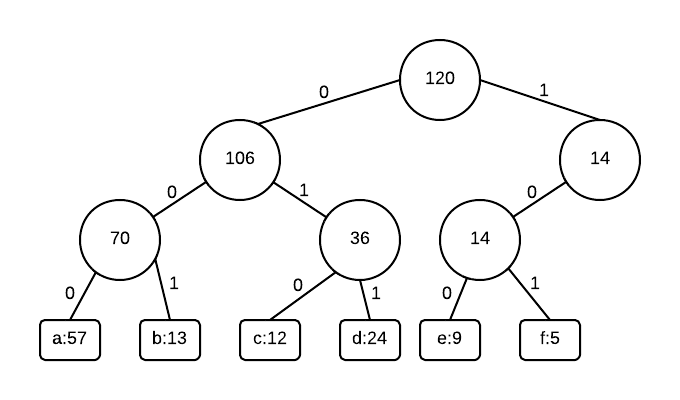
\includegraphics[width=100mm]{images/huff1.png}
\end{figure}

Tutti i caratteri sono foglie e sono allo stesso livello.
\linebreak
\linebreak
Esempio: codice a \textbf{lunghezza variabile}

\begin{center}
\begin{tabular}[htpd]{| l | c c c c c c |}

\hline
Carattere & a & b & c & d & e & f \\
Frequenza & 57 & 13 & 12 & 24 & 9 & 5 \\
Codice fisso & 0 & 101 & 100 & 111 & 1101 & 1100 \\
\hline
\end{tabular}
\end{center}

\begin{figure}[htpd]
\centering
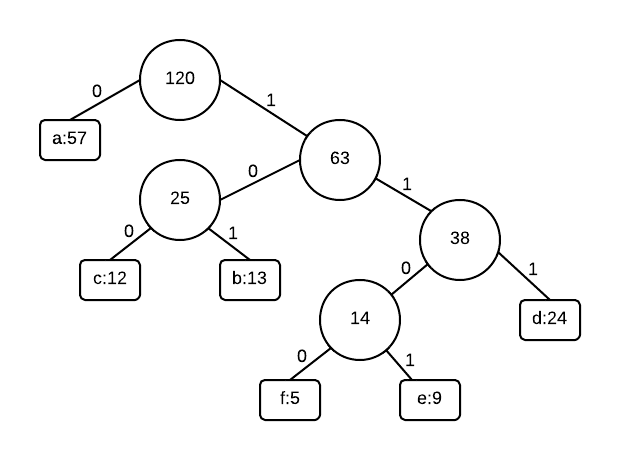
\includegraphics[width=100mm]{images/huff3.png}
\end{figure}

La lunghezza in bit del file codificato con il codice rappresentato da un albero $T$ è:

$$B(T)=\sum_{c\in\sum}f_cd_t(c)$$

dove $c\in\sum$ significa una sommatoria estesa a tutti i caratteri dell'alfabeto, $f_c$ è la frequenza del carattere $c$, $d_t(c)$ è la profondità della foglia che rappresenta il carattere $c$ nell'albero $T$.
\linebreak
\linebreak
\textbf{Nota}: assumiamo che l'alfabeto $\sum$ contenga almeno due caratteri. In caso contrario basata un numero per rappresentare il file: la sua lunghezza.

\subsection{Costruzione dell'albero del codice}

\begin{center}
\begin{tabular}[htpd]{| l | c c c c c c |}

\hline
Carattere & a & b & c & d & e & f \\
Frequenza & 57 & 13 & 12 & 24 & 9 & 5 \\
\hline
\end{tabular}
\end{center}

\begin{figure}[htpd]
\centering
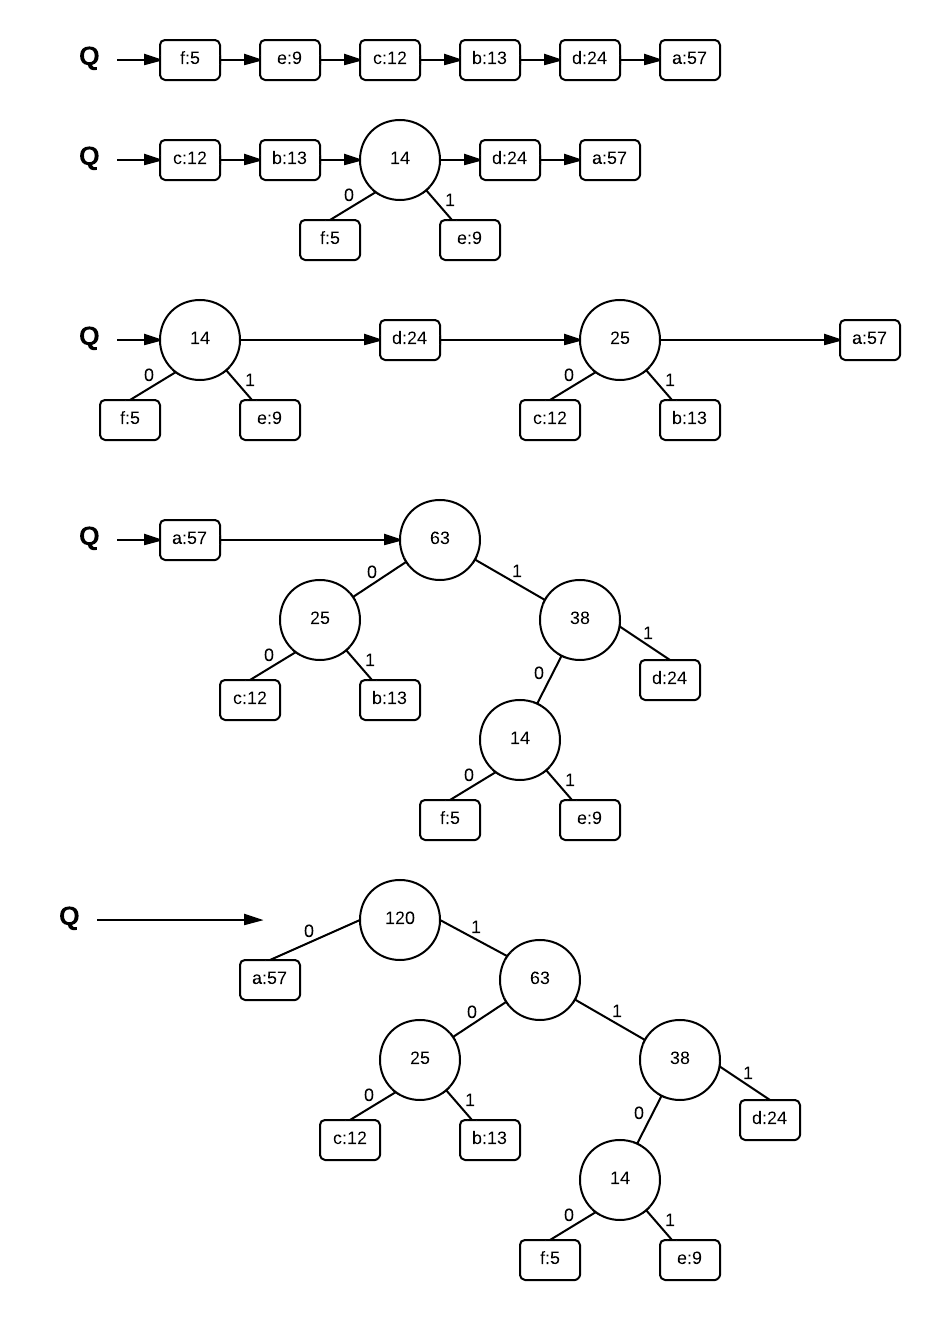
\includegraphics[width=100mm]{images/huff4.png}
\end{figure}

Vediamo di seguito l'algoritmo utilizzato per costruire l'albero:

\begin{lstlisting}[mathescape=true, caption=Huffman]

Huffman(c, f, n)
	Q = 0$\emptyset$
	for i=1 to n
		Push(Q, Nodo($f_i$, $c_i$))
	for j=n dowto 2
		x = ExtractMin(Q)
		y = ExtractMin(Q)
		Push(Q, Nodo(x,y))
	return ExtractMin(Q)

\end{lstlisting}

$Nodo(f,c)$ è il costruttore dei nodi foglia. $Nodo(x,y)$ è il costruttore dei nodi interni. La complessità dell'algoritmo è \textbf{$O(n\log n$}.
\linebreak
\linebreak
La tecnica di base per generare l'albero di un codice prefisso ottimo è quindi la seguente:

\begin{enumerate}

\item Ordinare la lista di caratteri per frequenza crescente;
\item Finchè la lista non contiene un solo elemento:
	\begin{enumerate}

	\item Estrarre i due caratteri con frequenza minore;
	\item Creare un nuovo albero che ha per figli i due caratteri del punto precedente e per radice la somma delle loro frequenze;
	\item Inserire l'albero nella lista (cancellando i fieli dalla lista).

	\end{enumerate}
\item Assegnare ad ogni carattere un codice secondo la definizione di albero del codice: un albero del codice è un albero binario le cui foglie sono i caratteri e una parola in codice viene interpretata come il cammino semplice dalla radice a quel carattere, dove 0 significa raggiungi il figlio sinistro e 1 significa raggiungi il figlio destro.
\end{enumerate}
